\documentclass[11pt]{article}
\usepackage[a4paper,left=1.5cm,right=1.5cm,top=1.5cm,bottom=1.5cm]{geometry}
\usepackage{fancyhdr}
\renewcommand{\headrulewidth}{1pt}
\fancyhead[C]{\textbf{[LINGI2132] Languages \& Translators}}
\fancyhead[L]{Assignment 1}
\fancyhead[R]{Group 55}

\usepackage[T1]{fontenc}
\usepackage[utf8]{inputenc}
\usepackage[english]{babel}
\usepackage{graphicx}
\usepackage{subcaption}
\usepackage{mathtools,amssymb}
\usepackage[binary-units=true,separate-uncertainty = true,multi-part-units=single]{siunitx}
\usepackage{float}
\setlength{\parskip}{1ex plus 0.5ex minus 0.2ex}
\newcommand{\hsp}{\hspace{20pt}}
\newcommand{\HRule}{\rule{\linewidth}{0.5mm}}
\graphicspath{{img/}}
\usepackage{caption}
\usepackage{textcomp}
\usepackage{array}
\usepackage{color}
\usepackage{tabularx,booktabs}
\usepackage{titlesec}
\usepackage{wrapfig}
\titlespacing{\section}{0pt}{\parskip}{-\parskip}
\titlespacing{\subsection}{0pt}{\parskip}{-\parskip}
\titlespacing{\subsubsection}{0pt}{\parskip}{-\parskip}
\pagestyle{fancy}
\usepackage{minted}
\usepackage{csquotes}
\usepackage[linktoc=all]{hyperref}
\hypersetup{breaklinks=true}

\begin{document}
\section{Division}
\label{sec:division}
The division operator is implemented as described in Chapter 1.5 of \cite{compilers}.
Tests were added (both passing and failing) in order to verify the correct execution of the program, as explained in Section~\ref{sec:test}.

\section{Remainder}
The remainder operator is implemented analoguously to the division operator, with the only real difference being that in \mintinline{java}{Scanner.getNextToken()}, the ``\mintinline{java}{%}'' token does not need to be treated separately, whereas the division symbol could indicate the start of a comment and special care needs to be taken.
For this reason, the code in this part was based on how multiplication is handled, whereas other parts are analogous with the division operator of Section~\ref{sec:division} and \cite{compilers}.
Tests are described in Section~\ref{sec:test}.

\section{Unary Addition}
The unary addition operator is implemented analoguously to the unary negation operator, which was already present in the code.
Its main difference from the binary operators described above is that instead of working in the \texttt{JBinaryExpression.java} file, changes need to be made to \texttt{JUnaryExpression.java}.
There is no dedicated JVM instruction for unary addition (contrary to unary negation, which uses \texttt{INEG}); for this reason, we use the \texttt{NOP} instruction, which does nothing and thus mimics unary addition.

\section{Palindrome}
To check a string for palindromicity, one traverses the string in both directions simultaneously, continuing as long as both traversed parts are the same.
If these substrings differ at some point, the function outputs an empty string and terminates, otherwise it continues until the pointers meet, and outputs the original string.
As discussed in \cite{complexity}, this algorithm is optimal from a complexity point of view.
To make this algorithm case-insensitive, the string is converted to lowercase before performing the comparison using the built-in Java \mintinline{java}{String} function \mintinline{java}{toLowerCase()}.

In order to check whether the middle of the string has been reached, the less-than operator (\(<\)) had to be implemented, which was done similarly to the greater-than operator which was already implemented.
Tests were also written for this operator, in order to verify its correctness, as explained in Section~\ref{sec:test}.

\section{Updates to Grammar}
The updates to the grammar and lexical grammar are given in Figures~\ref{fig:gram} and \ref{fig:lexical}.
\begin{figure}[H]
	\centering
	\begin{subfigure}[t]{0.5\textwidth}
		\centering
		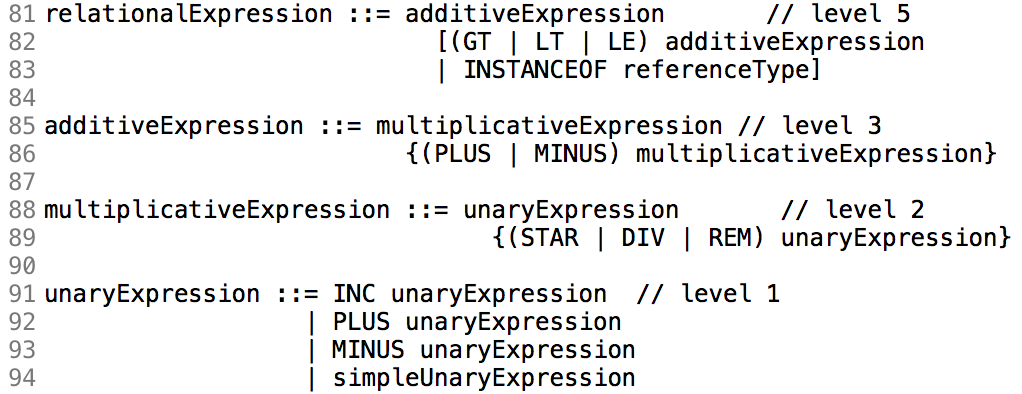
\includegraphics[width=0.87\linewidth]{img/grammar.png}
		\caption{Updated lines: 82, 85, 88, and 92}
		\label{fig:gram}
	\end{subfigure}\hfill
	\begin{subfigure}[t]{0.5\textwidth}
		\centering
		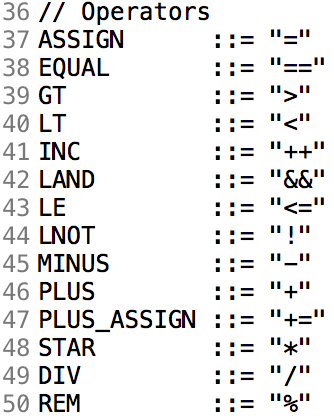
\includegraphics[width=0.27\linewidth]{img/lexicalgrammar.png}
		\caption{Updated: LT, DIV, and REM}
		\label{fig:lexical}
	\end{subfigure}
	\caption{Updates to the grammar (left) and lexical grammar (right) of \texttt{j-\(\)-}}
	\label{fig:grammar}
\end{figure}

\section{Testing Methodology}
\label{sec:test}
Tests were added in the same fashion as in \cite{compilers}, i.e., before implementing the functionality, and in the fashion of unit tests.
For division and remainder, these tests were really straightforward and make sure the behavior is as expected; all types of scenarios are verified.
For unary addition and less-than, adding tests was also fairly straightforward considering the similarities with the operators mentioned before.
Finally, to test the palindromicity check, all constraints on the output were checked in order to guarantee correct execution.

The various operators and functions were also verified on INGInious. obtaining a perfect score.

\begin{thebibliography}{9}
	\bibitem{compilers}
	Bill Campbell, Swami Iyer, and Bahar Akbal-Deliba\c s.
	\textit{Introduction to Compiler Construction in a Java World}.
	Chapman and Hall/CRC, Boca Raton, Florida, 2012.
	
	\bibitem{complexity}
	Fernando Pelliccioni.
	\href{http://componentsprogramming.com/palindromes/}{\textit{Palindromes and more}}.
	Components Programming, 2016.
\end{thebibliography}

\end{document}